% %%%% CUSTOM PREAMBLE
% \usepackage{./preamble}

% %% ADD MISC DEFINITIONS HERE %%%%%%%%%%%%%%%%%%%%%%%%%%%%%%%%%%%

% %%%%%%%%%%%%%%%%%%%%%%%%%%%%%%%%%%%%%%%%%%%%%%%%%%%%%
% %\addtolength{\topmargin}{-1cm}
% %\addtolength{\textheight}{2cm}

% \begin{document}


%\maketitle
\newpage
\noindent
\textbf{CS4268 AY2025-26 Sem 2}
\\
\noindent
Lecturer: Divesh Aggarwal
\hfill
Lecture 2                      %%% FILL IN LECTURE NUMBER HERE
\hfill
Date: January 22, 2026          %%% FILL IN LECTURE DATE HERE


\noindent
\rule{\textwidth}{1pt}

\medskip

\section{Hilbert Space and Quantum States}
The language of quantum mechanics is linear algebra. We shall assume some familiarity with it, but introduce a very useful bookkeeping tool -- Dirac's bra-ket notation.

\subsection{Hilbert Space}

Recall the notion of a Hilbert Space.
\begin{definition}[Hilbert Space]
A \textbf{Hilbert Space} $\mathcal{H}$ over $\mathbb{C}$ is a complete vector space over the complex numbers equipped with an inner product $\langle \cdot, \cdot \rangle : \mathcal{H} \times \mathcal{H} \to \mathbb{C}$ that satisfies:
\begin{itemize}
\item Conjugate symmetry: $\langle u, v \rangle = \overline{\langle v, u \rangle}$
\item Linearity in the second argument: $\langle u, \alpha v + \beta w \rangle = \alpha \langle u, v \rangle + \beta \langle u, w \rangle$ for $\alpha, \beta \in \mathbb{C}$
\item Positive definiteness: $\langle v, v \rangle \geq 0$ with equality if and only if $v = 0$
\end{itemize}
\end{definition}

\subsection{Dirac's Bra-Ket Notation}

Dirac's bra-ket notation:
\begin{definition}[Bra-ket Notation]
A \textbf{ket} $\ket{v}$ denotes a column vector in the Hilbert space $\mathcal{H}$.
\begin{itemize}
\item Basis vectors are denoted $\ket{0}, \ket{1}, \ldots, \ket{n-1}$ for an $n$-dimensional space.
\item A general vector can be written as a linear combination: $\ket{\psi} = \sum_{i} \alpha_i \ket{i}$ where $\alpha_i \in \mathbb{C}$.
\item A \textbf{bra} $\bra{v}$ denotes the conjugate transpose of $\ket{v}$, i.e., $\bra{v} = (\ket{v})^\dagger$, which is a row vector.
\item The inner product of two vectors $\ket{u}$ and $\ket{v}$ is written as $\langle u|v \rangle$.
\item Orthonormality of basis vectors: $\langle i|j \rangle = \delta_{ij}$.
\end{itemize}
\end{definition}

\begin{remark}[Conjugate Transpose as Bra]
Given a ket
\[
\ket{v} = \begin{pmatrix} v_1 \\ \vdots \\ v_d \end{pmatrix} \in \C^d,
\]
its bra is the conjugate transpose
\[
\bra{v} = (\ket{v})^\dagger = \big(v_1^*, \ldots, v_d^*\big).
\]
The inner product is therefore
\[
\langle u|v \rangle = u^\dagger v,
\]
which suppresses explicit matrix multiplication and should be read as ``bra-$u$ ket-$v$''.
\end{remark}

\begin{example}[Notations for Bases]
Dirac's notation unifies familiar notions of basis vectors:

\begin{itemize}
    \item \textbf{High school basis (in $\R^3$):}
    \[
        \hat{i} = \begin{pmatrix} 1 \\ 0 \\ 0 \end{pmatrix},\quad
        \hat{j} = \begin{pmatrix} 0 \\ 1 \\ 0 \end{pmatrix},\quad
        \hat{k} = \begin{pmatrix} 0 \\ 0 \\ 1 \end{pmatrix}
    \]

    \item \textbf{Linear algebra basis in $\R^d$ (standard basis):}
    \[
        e_1 = \begin{pmatrix} 1 \\ 0 \\ \vdots \\ 0 \end{pmatrix},\quad
        e_2 = \begin{pmatrix} 0 \\ 1 \\ \vdots \\ 0 \end{pmatrix},\quad
        \ldots,\quad
        e_d = \begin{pmatrix} 0 \\ 0 \\ \vdots \\ 1 \end{pmatrix}
    \]

    \item \textbf{Quantum computational basis in $\C^d$:}
    \[
        \ket{0} = \begin{pmatrix} 1 \\ 0 \\ 0 \\ \vdots \\ 0 \end{pmatrix},\quad
        \ket{1} = \begin{pmatrix} 0 \\ 1 \\ 0 \\ \vdots \\ 0 \end{pmatrix},\quad
        \ket{2} = \begin{pmatrix} 0 \\ 0 \\ 1 \\ \vdots \\ 0 \end{pmatrix},\quad
        \ldots,\quad
        \ket{d-1} = \begin{pmatrix} 0 \\ 0 \\ \vdots \\ 1 \end{pmatrix}
    \]
\end{itemize}

In an $n$-dimensional quantum system (e.g., qubit: $n=2$, qutrit: $n=3$, qudit: $n=d$), these vectors form the \emph{computational basis} $\{\ket{0},\ket{1},\ldots,\ket{n-1}\}$ and satisfy
\[
\langle i|j \rangle = \delta_{ij}.
\]
\end{example}

\begin{example}[Complex Vector Example]
Consider the vector
\[
\ket{v} = \frac{1}{13}
\begin{pmatrix}
3 + 4i \\
12i
\end{pmatrix}.
\]
Then the corresponding bra is
\[
\bra{v}
= \frac{1}{13}\big(3 - 4i,\; -12i\big),
\]
obtained by taking the conjugate transpose of the ket.
\end{example}

\subsection{Quantum States}

From now on everything is denoted in bra-ket notation.

In quantum mechanics a system is mathematically modelled by a suitable (to be determined from theory and experiment) Hilbert space. The quantum state representing the system is simply an element of this Hilbert space.
% \begin{definition}
%     Add quantum state as element of Hilbert space, as superposition of basis vectors, column vector representation. Add physical interpretation of the components $\alpha_i$ of the column vector.
% \end{definition}
\begin{definition}[Quantum State]
A \textbf{quantum state} $\ket{\psi}$ is an element of a Hilbert space $\mathcal{H}$ with unit norm, i.e., $\langle \psi|\psi \rangle = 1$.

For a quantum system with orthonormal basis $\{\ket{0}, \ket{1}, \ldots, \ket{n-1}\}$, any quantum state can be written as a superposition:
$$\ket{\psi} = \sum_{i=0}^{n-1} \alpha_i \ket{i} = \alpha_0 \ket{0} + \alpha_1 \ket{1} + \cdots + \alpha_{n-1} \ket{n-1}$$
where $\alpha_i \in \mathbb{C}$ are complex amplitudes satisfying the normalization condition $\sum_{i=0}^{n-1} |\alpha_i|^2 = 1$.

In column vector representation:
$$\ket{\psi} = \begin{pmatrix} \alpha_0 \\ \alpha_1 \\ \vdots \\ \alpha_{n-1} \end{pmatrix}.$$

\textbf{Physical Interpretation:} When we measure the quantum state $\ket{\psi}$ in the computational basis, the probability of observing outcome $i$ is $|\alpha_i|^2$. This is \textbf{Born's rule}.
\end{definition}

\begin{example}[Quantum States as Superpositions]
For a single qubit (2-dimensional quantum system):
\begin{itemize}
\item Computational basis states: $\ket{0} = \begin{pmatrix} 1 \\ 0 \end{pmatrix}$ and $\ket{1} = \begin{pmatrix} 0 \\ 1 \end{pmatrix}$

\item Superposition state: $\ket{+} = \frac{1}{\sqrt{2}}(\ket{0} + \ket{1}) = \frac{1}{\sqrt{2}}\begin{pmatrix} 1 \\ 1 \end{pmatrix}$

\item Another superposition: $\ket{-} = \frac{1}{\sqrt{2}}(\ket{0} - \ket{1}) = \frac{1}{\sqrt{2}}\begin{pmatrix} 1 \\ -1 \end{pmatrix}$

\item General qubit state: $\ket{\psi} = \alpha\ket{0} + \beta\ket{1}$ where $|\alpha|^2 + |\beta|^2 = 1$
\end{itemize}
The states $\ket{+}$ and $\ket{-}$ form the Hadamard basis (also called the $X$-basis or plus-minus basis).
\end{example}

Of course, we know the basis of a (nontrivial) Hilbert space is not unique. We could choose to represent states w.r.t. different bases, so the corresponding column vectors would have different physical interpretations.

\section{Measurements in different bases and the Elitzur-Vaidman Test}
\subsection{Measurements in Different Bases}
Up until now, we have only considered measurements with respect to the standard basis ($\{ \ket{0}, \ket{1} \}$ in the $2$ dimensional case). However, we are not restricted to just measuring in the standard basis and can use any valid set of orthonormal basis states as the measurement basis. Let us now consider the problem of making measurements with respect to different bases.
\begin{example}[Measurement with respect to Different Bases]
Consider a qubit in state $\ket{+} = \frac{1}{\sqrt{2}}(\ket{0} + \ket{1})$.

\textbf{Measurement w.r.t. computational basis $\{\ket{0}, \ket{1}\}$}:
\begin{itemize}
\item $\pr(\text{measure} \ket{0}) = |\frac{1}{\sqrt{2}}|^2 = \frac{1}{2}$,
\item $\pr(\text{measure} \ket{1}) = |\frac{1}{\sqrt{2}}|^2 = \frac{1}{2}$.
\end{itemize}

\textbf{Measurement w.r.t. Hadamard basis $\{\ket{+}, \ket{-}\}$}:

First, express $\ket{+}$ in the new basis. Since $\ket{0} = \frac{1}{\sqrt{2}}(\ket{+} + \ket{-})$ and $\ket{1} = \frac{1}{\sqrt{2}}(\ket{+} - \ket{-})$, we have:
$$\ket{+} = \frac{1}{\sqrt{2}}(\ket{0} + \ket{1}) = \frac{1}{\sqrt{2}}\left[\frac{1}{\sqrt{2}}(\ket{+} + \ket{-}) + \frac{1}{\sqrt{2}}(\ket{+} - \ket{-})\right] = 1 \cdot \ket{+} + 0 \cdot \ket{-}.$$

Thus
\begin{itemize}
\item $\pr(\text{measure} \ket{+}) = |1|^2 = 1$,
\item $\pr(\text{measure} \ket{-}) = |0|^2 = 0$.
\end{itemize}

\textbf{Key insight:} When we measure $\ket{+}$ in the Hadamard basis $\{\ket{+}, \ket{-}\}$, the coefficient of $\ket{+}$ is 1 and the coefficient of $\ket{-}$ is 0. This makes intuitive sense: if the system is already in state $\ket{+}$ and we measure in the $\{\ket{+}, \ket{-}\}$ basis, we are guaranteed to get the outcome $\ket{+}$. Thus, the same quantum state gives different measurement outcomes depending on the measurement basis.
\end{example}

\subsection{Elitzur-Vaidman Bomb-Tester}
Now let us consider the following thought experiment. Suppose we are given a box that is either a DUD or a bomb. We want to figure out which box we are given without triggering an explosion. The behaviour of the two possible boxes is shown below:
% Classical option and preliminary quantum option. Conclusions from these options.
\begin{center}
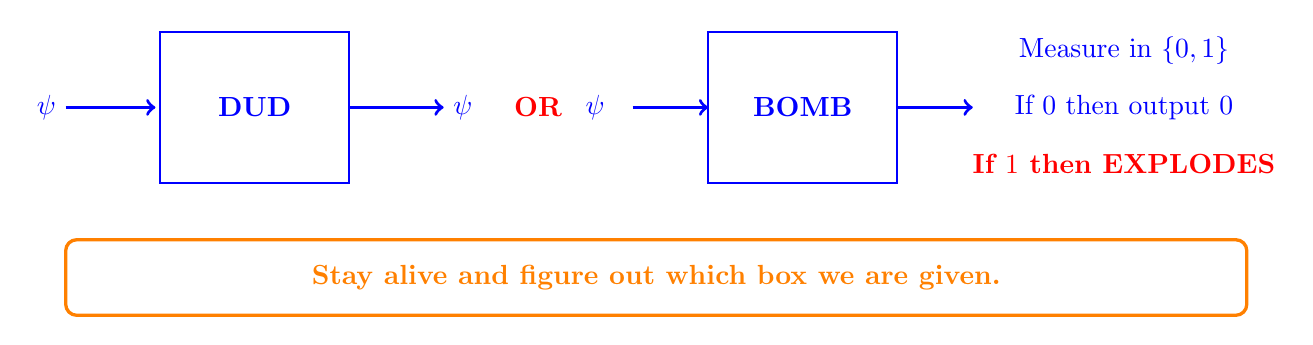
\begin{tikzpicture}[scale=1.2]
% Photon input
\draw[->, very thick, blue] (-1,0) -- (-0.05,0);
\node[left, blue] at (-1,0) {$\ket{\psi}$};

% First box - DUD
\draw[thick, blue] (0,-0.8) rectangle (2,0.8);
\node[blue] at (1,0) {\textbf{DUD}};

% Arrow from DUD
\draw[->, very thick, blue] (2,0) -- (3,0);
\node[right, blue] at (3,0) {$\ket{\psi}$};

% OR text with more space
\node[red, font=\bfseries] at (4.0,0) {OR};

% Arrow to bomb with spacing
\draw[->, very thick, blue] (5.0,0) -- (5.8,0);
\node[right, blue] at (4.4,0) {$\ket{\psi}$};

% Second box - BOMB
\draw[thick, blue] (5.8,-0.8) rectangle (7.8,0.8);
\node[blue] at (6.8,0) {\textbf{BOMB}};

% Arrow from BOMB to right
\draw[->, very thick, blue] (7.8,0) -- (8.6,0);

% Measure text (no arrow, just text aligned to the right)
\node[blue, align=left] at (10.2,0.6) {Measure in $\{\ket{0}, \ket{1}\}$};

% Outcomes
\node[blue, align=left] at (10.2, 0) {If $\ket{0}$ then output $\ket{0}$};
\node[red, align=left, font=\bfseries] at (10.2,-0.6) {If $\ket{1}$ then EXPLODES};

% Goal box at bottom
\draw[orange, very thick, rounded corners] (-1,-1.4) rectangle (11.5,-2.2);
\node[orange, font=\bfseries] at (5.25,-1.8) {Stay alive and figure out which box we are given.};
\end{tikzpicture}
\end{center}

Some preliminary options that comes to mind are sending $\ket{0}$ or $\ket{+}$ through the unknown box, and then measure the output from the box. Let us examine what happens in each of these cases.

\textbf{Classical Strategy:}

If we send $\ket{0}$, we are unable to identify if it is a dud or a bomb as the output is the same. If we send $\ket{1}$:
\begin{itemize}
\item No explosion $\Rightarrow$ it's a dud!
\item Bomb explodes $\Rightarrow$ it's a bomb! (but you dead)
\end{itemize}

\textit{Conclusion:} Classically impossible to distinguish dud/bomb without triggering an explosion.

\textbf{Preliminary Quantum Strategy:}

Send in $\ket{\psi} = \ket{+}$ and measure w.r.t. $\{\ket{+}, \ket{-}\}$.

\textit{Case 1: Dud bomb}

If it's a dud, we will always see $\ket{+}$ because 100\% of the amplitude is on $\ket{+}$.

\begin{center}
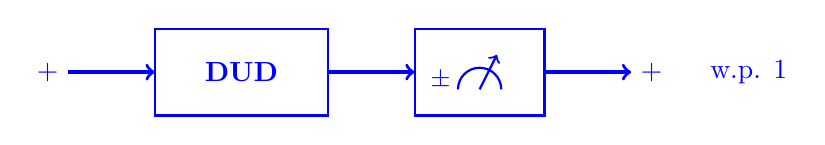
\begin{tikzpicture}[scale=1.1]
\draw[->, very thick, blue] (0,0) -- (1,0);
\node[left, blue] at (0,0) {$\ket{+}$};
\draw[thick, blue] (1,-0.5) rectangle (3,0.5);
\node[blue] at (2,0) {\textbf{DUD}};
\draw[->, very thick, blue] (3,0) -- (4,0);
\draw[thick, blue] (4,-0.5) rectangle (5.5,0.5);
% Measurement device with arc and arrow
\node[blue, font=\small] at (4.3,-0.1) {$\pm$};
\draw[blue, thick] (4.5,-0.2) arc[start angle=180, end angle=0, radius=0.25];
\draw[blue, thick, ->] (4.75,-0.2) -- (4.95,0.2);
\draw[->, very thick, blue] (5.5,0) -- (6.5,0);
\node[right, blue] at (6.5,0) {$\ket{+}$};
\node[right, blue] at (7.3,0) {w.p. 1};
\end{tikzpicture}
\end{center}

\textit{Case 2: Working bomb}

Three possible outcomes:
\begin{itemize}
\item Bomb measures $\ket{0}$ and explodes (with probability $\frac{1}{2}$).
\item Bomb measures $\ket{1}$ and does not explode:
\begin{itemize}
\item We observe $\ket{+}$ (with probability $\frac{1}{4}$): inconclusive (could be dud or working)
\item We observe $\ket{-}$ (with probability $\frac{1}{4}$): Working bomb identified!
\end{itemize}
\end{itemize}

\begin{center}
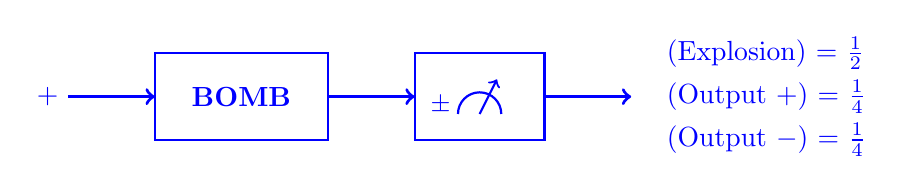
\begin{tikzpicture}[scale=1.1]
\draw[->, very thick, blue] (0,0) -- (1,0);
\node[left, blue] at (0,0) {$\ket{+}$};
\draw[thick, blue] (1,-0.5) rectangle (3,0.5);
\node[blue] at (2,0) {\textbf{BOMB}};
\draw[->, very thick, blue] (3,0) -- (4,0);
\draw[thick, blue] (4,-0.5) rectangle (5.5,0.5);
% Measurement device with arc and arrow
\node[blue, font=\small] at (4.3,-0.1) {$\pm$};
\draw[blue, thick] (4.5,-0.2) arc[start angle=180, end angle=0, radius=0.25];
\draw[blue, thick, ->] (4.75,-0.2) -- (4.95,0.2);
\draw[->, very thick, blue] (5.5,0) -- (6.5,0);
\node[blue, align=left, anchor=west] at (6.8,0.5) {$\pr$(Explosion) = $\frac{1}{2}$};
\node[blue, align=left, anchor=west] at (6.8,0) {$\pr$(Output $\ket{+}$) = $\frac{1}{4}$};
\node[blue, align=left, anchor=west] at (6.8,-0.5) {$\pr$(Output $\ket{-}$) = $\frac{1}{4}$};
\end{tikzpicture}
\end{center}

If we observe $\ket{-}$, we know it is a bomb because: with a dud, we get $\ket{+}$ all the time (with probability 1).

\textit{Conclusion:} $\frac{1}{4}$ success rate for identifying working bomb without explosion. 

\textbf{Can we improve upon this?} Yes.
First, but first let us make a brief detour into the notion of rotations (more generally, unitaries later on) on quantum states.

% \begin{definition}
%     Add material on rotations on a single qubit.
% \end{definition}
\subsection{Rotations and Reflections}

\paragraph{Rotations}

\begin{definition}[Rotations on a Single Qubit]
For any $\theta$, we can build a physical device that rotates a qubit by angle $\theta$. Consider a transformation that rotates the quantum state by a small angle $\theta$. Starting from $\ket{0}$, we apply a rotation:
$R(\theta): \ket{0} \mapsto \cos(\theta)\ket{0} + \sin(\theta)\ket{1}$

$$\ket{0} \to \begin{pmatrix} \cos\theta \\ \sin\theta \end{pmatrix}$$

$$\ket{1} \to \begin{pmatrix} \cos(\frac{\pi}{2} + \theta) \\ \sin(\frac{\pi}{2} + \theta) \end{pmatrix} = \begin{pmatrix} -\sin\theta \\ \cos\theta \end{pmatrix}$$

\begin{center}
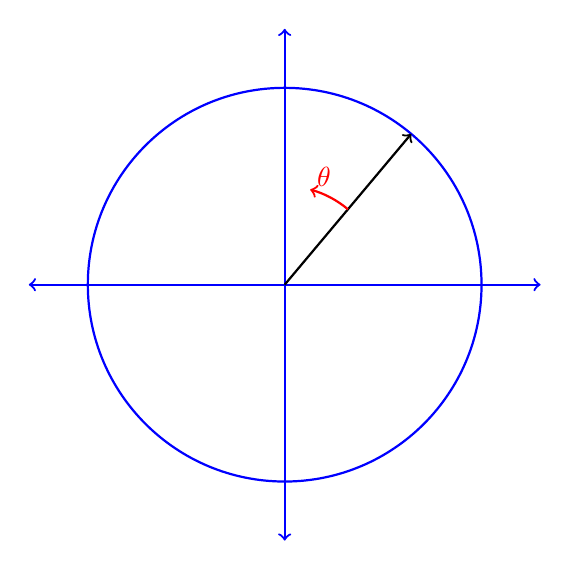
\begin{tikzpicture}[scale=2.5]
% Draw circle
\draw[thick, blue] (0,0) circle (1);
% Draw axes with arrows on both ends
\draw[thick, blue, <->] (-1.3,0) -- (1.3,0);
\draw[thick, blue, <->] (0,-1.3) -- (0,1.3);
% Draw vector at angle
\draw[thick, black, ->] (0,0) -- ({cos(50)},{sin(50)});
% Draw curved rotation arrow starting FROM the black arrow curving left, ending before vertical axis
\draw[thick, red, ->] ({0.5*cos(50)},{0.5*sin(50)}) arc (50:75:0.5);
\node[red] at (0.2,0.55) {$\theta$};
\end{tikzpicture}
\end{center}

For a general state $\alpha\ket{0} + \beta\ket{1}$, it gets transformed to:

\begin{align*}
\alpha\ket{0} + \beta\ket{1} &\to \alpha\begin{pmatrix} \cos\theta \\ \sin\theta \end{pmatrix} + \beta\begin{pmatrix} -\sin\theta \\ \cos\theta \end{pmatrix}\\
&\quad= \begin{pmatrix} \cos\theta & -\sin\theta \\ \sin\theta & \cos\theta \end{pmatrix} \begin{pmatrix} \alpha \\ \beta \end{pmatrix}
\
\end{align*}
where $\begin{pmatrix} 1 \\ 0 \end{pmatrix}$ goes to the vector $\begin{pmatrix} \cos\theta \\ \sin\theta \end{pmatrix}$ and $\begin{pmatrix} 0 \\ 1 \end{pmatrix}$ goes to the vector $\begin{pmatrix} -\sin\theta \\ \cos\theta \end{pmatrix}$.

Any state $\ket{\psi}$ gets transformed to $R_\theta\ket{\psi}$, where:
$$R_\theta = \begin{pmatrix} \cos\theta & -\sin\theta \\ \sin\theta & \cos\theta \end{pmatrix}$$

\textbf{Note:} 
\begin{itemize}
\item $\alpha$ and $\beta$ may be complex numbers.
\item Viewing $R_\theta$ as a rotation may only be intuitive for real amplitudes.
\end{itemize}
\end{definition}

\textbf{Measuring w.r.t. $\ket{u}, \ket{v}$ basis via rotation:}

\begin{center}
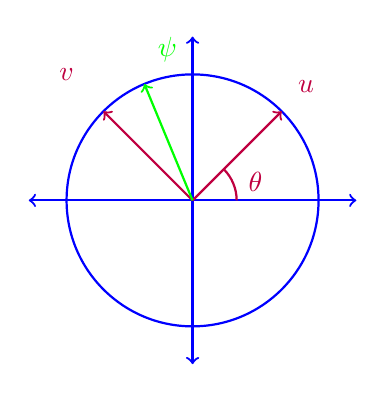
\begin{tikzpicture}[scale=1.6]

% Circle
\draw[thick, blue] (0,0) circle (1);

% Axes with arrow tips
\draw[thick, blue, <->] (-1.3,0) -- (1.3,0);
\draw[thick, blue, <->] (0,-1.3) -- (0,1.3);

\draw[thick, purple, ->] (0,0) -- ({cos(45)},{sin(45)});
\node[purple] at (0.9,0.9) {$\ket{u}$};

\draw[thick, purple, ->] (0,0) -- ({cos(135)},{sin(135)});
\node[purple] at (-1.0,1.0) {$\ket{v}$};

% |psi> vector near vertical axis but slightly right (100 degrees)
\draw[thick, green, ->] (0,0) -- ({cos(112.5)},{sin(112.5)});
\node[green] at (-0.2,1.2) {$\ket{\psi}$};

% Angle theta between horizontal and u
\draw[thick, purple] (0.35,0) arc (0:45:0.35);
\node[purple] at (0.5,0.15) {$\theta$};

\end{tikzpicture}
\end{center}

$$\ket{u} = R_\theta\ket{0}$$
$$\ket{v} = R_\theta\ket{1}$$

For any state:
\begin{align*}
    \ket{\psi} &= \alpha\ket{u} + \beta\ket{v}\\
    &= \alpha \cdot R_\theta\ket{0} + \beta \cdot R_\theta\ket{1}
\end{align*}


\textbf{How to measure in $\ket{u}, \ket{v}$ while actually measuring in standard basis?}

Apply $R_{-\theta}$ to $\ket{\psi}$:
$$R_{-\theta}\ket{\psi} = \alpha\ket{0} + \beta\ket{1}$$

Then measure in $\{\ket{0}, \ket{1}\}$:
\begin{itemize}
\item $\ket{0}$ with probability $|\alpha|^2$ $\rightarrow$ output $\ket{u}$
\item $\ket{1}$ with probability $|\beta|^2$ $\rightarrow$ output $\ket{v}$.
\end{itemize}

\paragraph{Reflections}

\textbf We can also build reflectors along any axis.

\textbf{Example 1:} Reflection along diagonal axis

\begin{center}
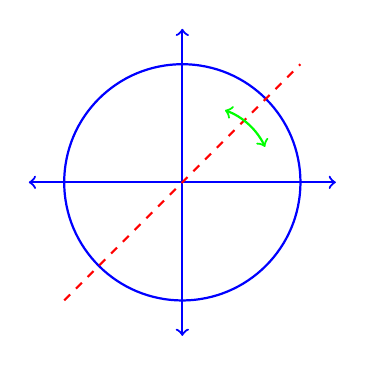
\begin{tikzpicture}[scale=1.5]
% Draw circle
\draw[thick, blue] (0,0) circle (1);
% Draw axes with arrows on both ends
\draw[thick, blue, <->] (-1.3,0) -- (1.3,0);
\draw[thick, blue, <->] (0,-1.3) -- (0,1.3);
% Draw diagonal reflection axis (red dashed)
\draw[thick, red, dashed] (-1,-1) -- (1,1);
% Add green curved arrow showing reflection
\draw[thick, green, <->] (0.7,0.3) arc (25:70:0.6);
\end{tikzpicture}
\end{center}

Reflection transformations:
$$\begin{pmatrix} 1 \\ 0 \end{pmatrix} \to \begin{pmatrix} 0 \\ 1 \end{pmatrix}, \quad \begin{pmatrix} 0 \\ 1 \end{pmatrix} \to \begin{pmatrix} 1 \\ 0 \end{pmatrix}$$
$$\ket{0} \to \ket{1}, \quad \ket{1} \to \ket{0}$$

For a general state:
$$\begin{pmatrix} \alpha \\ \beta \end{pmatrix} \text{ gets transformed to } \begin{pmatrix} \beta \\ \alpha \end{pmatrix}$$

\textbf{NOT operation:} 
$$\ket{\psi} = \begin{pmatrix} \alpha \\ \beta \end{pmatrix} \text{ maps to } \begin{pmatrix} 0 & 1 \\ 1 & 0 \end{pmatrix}\begin{pmatrix} \alpha \\ \beta \end{pmatrix}$$

\textbf{Example 2:} Hadamard gate (reflection along different axis)

\begin{center}
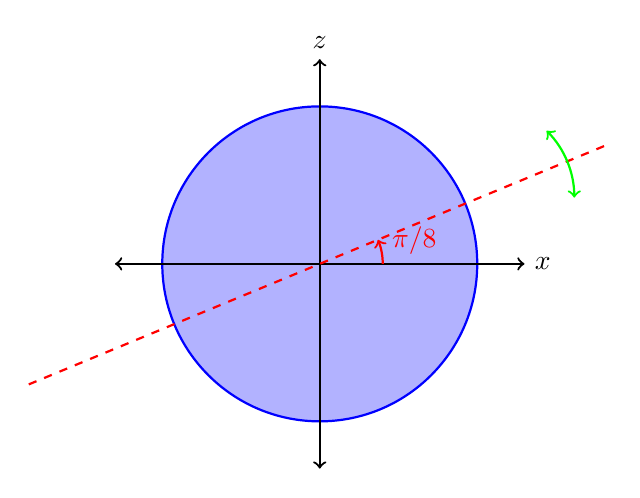
\begin{tikzpicture}[scale=2]
% Draw filled circle
\fill[blue!30] (0,0) circle (1);
\draw[thick, blue] (0,0) circle (1);
% Draw axes with arrows on both ends
\draw[thick, black, <->] (-1.3,0) -- (1.3,0) node[right] {$x$};
\draw[thick, black, <->] (0,-1.3) -- (0,1.3) node[above] {$z$};
% Draw Hadamard reflection axis at pi/8 (22.5 degrees) extended more beyond circle
\draw[thick, red, dashed] ({-2.0*cos(22.5)},{-2.0*sin(22.5)}) -- ({2.0*cos(22.5)},{2.0*sin(22.5)});
% Add green curved arrow centered on the dotted axis at distance 1.1
% Arc from (22.5-22.5) to (22.5+22.5) degrees, radius 0.6, centered at point on axis
\draw[thick, green, <->] ({1.1*cos(22.5)+0.6*cos(0)},{1.1*sin(22.5)+0.6*sin(0)}) arc (0:45:0.6);
% Draw arc showing pi/8 angle from horizontal axis to dashed line
\draw[thick, red, ->] (0.4,0) arc (0:22.5:0.4);
\node[red] at (0.60,0.15) {$\pi/8$};
\end{tikzpicture}
\end{center}

Hadamard transformations:
$$\ket{0} \text{ maps to } \ket{+}$$
$$\ket{1} \text{ maps to } \ket{-}$$

$$\psi = \begin{pmatrix} \alpha \\ \beta \end{pmatrix} \text{ is mapped to } \begin{pmatrix} \frac{1}{\sqrt{2}} & \frac{1}{\sqrt{2}} \\ \frac{1}{\sqrt{2}} & -\frac{1}{\sqrt{2}} \end{pmatrix}\begin{pmatrix} \alpha \\ \beta \end{pmatrix}$$

This is labeled the Hadamard gate and is arguably the most important transformation in quantum computing.

\subsection{Elitzur-Vaidman Revisited}

\textbf{Improved Quantum Strategy via small-angle rotations (Quantum Zeno effect)}
We now show how to make the explosion probability arbitrarily small. Let $\varepsilon = \frac{\pi}{2N}>0$ be a small angle, i.e. $N$ is large. Define the rotation operator
\[
R_\varepsilon=
\begin{pmatrix}
\cos\varepsilon & -\sin\varepsilon\\
\sin\varepsilon & \cos\varepsilon
\end{pmatrix}.
\]
Starting from $\ket{0}$, we perform the following protocol:

\begin{enumerate}
    \item Apply $R_\varepsilon$.
    \item Send the qubit through the unknown box.
    \item If no explosion occurs, repeat the above steps $N$ times.
    \item Finally, measure in the computational basis.
\end{enumerate}

\textbf{Dud:} Since $N=\frac{\pi}{2\varepsilon}$, in the dud case the cumulative rotation is
\[
R_\varepsilon^N = R_{\pi/2},
\]
which maps $\ket{0}$ close to $\ket{1}$. Thus after $N$ rounds the state is approximately $\ket{1}$, and a final measurement yields outcome $\ket{1}$ with full certainty.

\textbf{Working Bomb:} After a single application of $R_\varepsilon$ the state becomes $\cos\varepsilon\ket{0}+\sin\varepsilon\ket{1}$. The box then measures in the computational basis. The probability of explosion in that round is $\sin^2\varepsilon \leq \varepsilon^2$. If no explosion occurs, the state collapses back to $\ket{0}$, and the process repeats.

By the union bound, the probability of at least one explosion over $N$ rounds is upper-bounded by $N\varepsilon^2=\frac{\pi}{2}\varepsilon$, tending to $0$ as $\varepsilon \to 0$. Meanwhile, if no explosion occurs for any of the $N$ rounds, the final measurement yields $\ket{0}$, in stark contrast to the dud case, which yields $\ket{1}$. Thus by choosing $\varepsilon$ sufficiently small, we can distinguish a live bomb from a dud
with arbitrarily high confidence, while making the probability of explosion arbitrarily small.

In a nutshell, using this quantum Zeno strategy we have
\begin{align*}
    \Pr(\text{observe } \ket{1}\,|\,\text{ DUD }) &= 1\\
    \Pr(\text{observe } \ket{0}\,|\,\text{ BOMB }) &\geq 1 - \frac{\pi}{2}\varepsilon.
\end{align*}


\section{Unitary Operations}
We have already seen some operations like the \textbf{NOT} operation and the \textbf{Hadamard} operation. We will now understand what kind of transformations are allowed on quantum states. The transformations that are physically allowed on quantum states are called unitary transformations (or operations). Intuitively, unitaries preserve the `length' of quantum states, thus preserving probability densities.

\textbf{Quantum Mechanics Law 3:} Quantum states can be transformed (without losing information) via \textbf{unitary transformations}.

\begin{definition}[Unitary Matrices]
    A linear transformation $U : \mathcal{H} \to \mathcal{H}$ on a complex Hilbert space is called \textbf{unitary} if it preserves the norm of every state. That is,
    \[
        \| U \ket{\vec{\psi}} \|^2 = \| \ket{\vec{\psi}} \|^2
        \quad \text{for all } \ket{\vec{\psi}} \in \mathcal{H}.
    \]
\end{definition}

Here are a few examples of unitary matrices:
\begin{example}[Examples of Unitary Matrices]\hfill
\begin{enumerate}
\item \textbf{Identity:} $I = \begin{pmatrix} 1 & 0 \\ 0 & 1 \end{pmatrix}$

\item \textbf{Pauli-X (NOT gate):} $X = \begin{pmatrix} 0 & 1 \\ 1 & 0 \end{pmatrix}$

Effect: $X\ket{0} = \ket{1}$ and $X\ket{1} = \ket{0}$ (bit flip)

\item \textbf{Pauli-Y:} $Y = \begin{pmatrix} 0 & -i \\ i & 0 \end{pmatrix}$

\item \textbf{Pauli-Z (phase flip):} $Z = \begin{pmatrix} 1 & 0 \\ 0 & -1 \end{pmatrix}$

Effect: $Z\ket{0} = \ket{0}$ and $Z\ket{1} = -\ket{1}$

\item \textbf{Hadamard gate:} $H = \frac{1}{\sqrt{2}}\begin{pmatrix} 1 & 1 \\ 1 & -1 \end{pmatrix}$

Effect: Creates equal superpositions
\begin{align*}
H\ket{0} &= \frac{1}{\sqrt{2}}(\ket{0} + \ket{1}) = \ket{+} \\
H\ket{1} &= \frac{1}{\sqrt{2}}(\ket{0} - \ket{1}) = \ket{-}
\end{align*}

Note: $H^2 = I$ (Hadamard is self-inverse).

\item \textbf{Phase gate (S gate):} $S = \begin{pmatrix} 1 & 0 \\ 0 & i \end{pmatrix}$

\item \textbf{T gate ($\pi/8$ gate):} $T = \begin{pmatrix} 1 & 0 \\ 0 & e^{i\pi/4} \end{pmatrix}$

\item \textbf{Rotation gates:}
$R_z(\theta) = \begin{pmatrix} e^{-i\theta/2} & 0 \\ 0 & e^{i\theta/2} \end{pmatrix}$
\end{enumerate}
\end{example}






\subsection{Properties of Unitaries}
Let us present the various characterizations of unitary matrices.

\begin{proposition}[Basic Properties of Unitary Matrices]\hfill
\begin{enumerate}
\item \textbf{Preservation of inner products and norms)}: for any $\ket{v}, \ket{w}$:
$\langle Uv | Uw \rangle = \langle v | U^\dagger U | w \rangle = \langle v | w \rangle$. In particular, $\|U\ket{v}\|^2 = \|\ket{v}\|^2$.

\item \textbf{Preservation of angles}: Since $\cos(\theta) := \frac{\langle v | w \rangle}{\|v\|\|w\|}$ and unitary transformations preserve both inner products and norms, the angle between any two vectors is also preserved.

\item \textbf{Eigenvalues lie on unit circle:} If $U\ket{v} = \lambda\ket{v}$, then $|\lambda| = 1$.
\textit{Proof:} $\|\ket{v}\|^2 = \|U\ket{v}\|^2 = \|\lambda\ket{v}\|^2 = |\lambda|^2\|\ket{v}\|^2$, so $|\lambda| = 1$.

\item \textbf{Determinant has unit modulus:} $|\det(U)| = 1$. \textit{Proof:} take determinants on both sides of $U^\dag U=I$.

\item \textbf{Composition of unitaries is unitary:} If $U, V$ are unitary, then $(UV)^\dagger(UV) = V^\dagger U^\dagger U V = V^\dagger V = I$.

\item \textbf{Inverse is unitary:} If $U$ is unitary, so is $U^\dagger = U^{-1}$.

\item \textbf{Reversibility:} Quantum evolution is reversible. Given $\ket{\psi'} = U\ket{\psi}$, we can always recover $\ket{\psi} = U^{-1}\ket{\psi'}= U^\dagger\ket{\psi'}$.

\item \textbf{Square roots exist:} Every unitary $U$ has a square root $W$, which is also unitary, such that $W^2 = U$. This allows for fractional quantum operations.

\textit{Example:} Consider the NOT gate (Pauli-X): $X = \begin{pmatrix} 0 & 1 \\ 1 & 0 \end{pmatrix}$. Its square root is:
$$\sqrt{X} = \frac{1}{2}\begin{pmatrix} 1+i & 1-i \\ 1-i & 1+i \end{pmatrix}$$

We can verify: $\sqrt{X} \cdot \sqrt{X} = \frac{1}{4}\begin{pmatrix} 1+i & 1-i \\ 1-i & 1+i \end{pmatrix}\begin{pmatrix} 1+i & 1-i \\ 1-i & 1+i \end{pmatrix} = \begin{pmatrix} 0 & 1 \\ 1 & 0 \end{pmatrix} = X$

On the Bloch sphere, $\sqrt{X}$ represents a rotation halfway to the full NOT operation.
\end{enumerate}
\end{proposition}


\subsection{Classical Analogue of Unitary Transformations}
It is instructive to compare unitary evolution in quantum mechanics with the way probability distributions evolve in classical randomized processes. In the classical setting, a system with $d$ possible outcomes can be represented by a probability vector
\[
p =
\begin{bmatrix}
p_1\\
p_2\\
\vdots\\
p_d
\end{bmatrix},
\qquad
p_i \ge 0,
\qquad
\sum_{i=1}^d p_i = 1.
\]

A randomized procedure transforms $p$ into a new distribution $p'$ via multiplication by a matrix $M$:
\[
p' = Mp.
\]
To preserve total probability, such a matrix must be column-stochastic, meaning its entries are non-negative and each column sums to $1$:
\[
M_{ij}\ge 0
\qquad\text{and}\qquad
\sum_{i=1}^d M_{ij} = 1 \ \ \text{for all } j.
\]

We now illustrate this with a classical example.

Consider the following random process: we roll a fair die; if the outcome is odd, we toss a fair coin; if it's heads, add $1$ to the outcome of the fair die.

Let the state space be $\{1,2,3,4,5,6\}$, and start from the uniform distribution
\[
p=
\begin{bmatrix}
\frac16\\
\frac16\\
\frac16\\
\frac16\\
\frac16\\
\frac16
\end{bmatrix}.
\]
The transformation implemented by the above procedure is captured by the column-stochastic matrix
\[
M=
\begin{bmatrix}
\frac12 & 0 & 0 & 0 & 0 & 0\\
\frac12 & 1 & 0 & 0 & 0 & 0\\
0 & 0 & \frac12 & 0 & 0 & 0\\
0 & 0 & \frac12 & 1 & 0 & 0\\
0 & 0 & 0 & 0 & \frac12 & 0\\
0 & 0 & 0 & 0 & \frac12 & 1
\end{bmatrix},
\qquad
p' = Mp.
\]
Starting from an odd face $1,3,5$, the coin toss either keeps the value (tails) or moves it to the next even face (heads), giving the $\frac12$--$\frac12$ split in the corresponding column. Starting from an even face $2,4,6$, the value stays unchanged, which is why the corresponding column has a single $1$.

This classical picture is quite similar to quantum evolution in that both are linear transformations on vectors. However, there are key differences.

First, classical stochastic evolution preserves the $\ell_1$ norm,
\[
\|p'\|_1 = \|p\|_1 = 1,
\]
whereas quantum evolution preserves the $\ell_2$ norm,
\[
\|U\ket{\psi}\|_2 = \|\ket{\psi}\|_2.
\]

Second, classical stochastic transformations are generally not reversible: a column-stochastic matrix need not be invertible, and even when it is invertible, its inverse typically does not have non-negative entries and therefore does not correspond to a valid stochastic process. In contrast, every unitary matrix is reversible, with inverse $U^\dagger$ as seen in the characterisation. This reversibility is one of the fundamental distinctions between classical and quantum dynamics.




